\section{引言}
基金中基金(fund of funds,简称FOF)是指投资于其他基金组合的基金.在欧美市场,基金中基金已经发展成为数量和规模均较大的一类成熟的理财产品.在美国市场上, FOF市场总资产在1995年初仅有3891.54百万美元,到2016年底已发展为1439637.04百万美元,年均增长率高达30.84\%.

2016年9月,中国证券监督管理委员会发布《公开募集证券投资基金运作指引第2号------基金中基金指引》,标志着公募基金行业迎来创新品种FOF,并由此进入FOF发展的全新时代.
\subsection{基金中基金的起源}

基金中基金起源于上世纪70年代,最初是以其他私募股权基金(private equity fund)为投资的标的.这是因为私募股权基金往往设置有非常高的投资门槛,单笔投资的资金规模巨大,并且要求参与者为合格投资者,这使得许多有意愿投资私募股权基金的个人投资者被拒之门外.而PE FOF作为渠道,解决了这个问题,使得个人投资者可以通过投资PE FOF,即间接地投资一篮子私募股权基金,来分享风险投资可能带来的高收益.

与中国市场不同,美国法律对于没有明确规定禁止的事情,默认为许可,而在中国,公民仅能做法律允许的事.这使得美国资本市场的创新能力非常强大,非常有利于全新产品的创立.

\subsection{基金中基金的成熟契机}

1987年10月19日,美国股票市场在经历了两年的牛市之后,遭受到一次巨大的股灾,这也是历史上继1929年经济危机后第二次全球经济危机.道琼斯指数单日跌幅达22\%,恒生指数暴跌11\%,这促使投资者开始思考如何根据市场的不同情况配置不同种类的基金,分散标的,减小风险.

\begin{figure}[ht]
\begin{minipage}[ht]{0.47\textwidth}
\centering
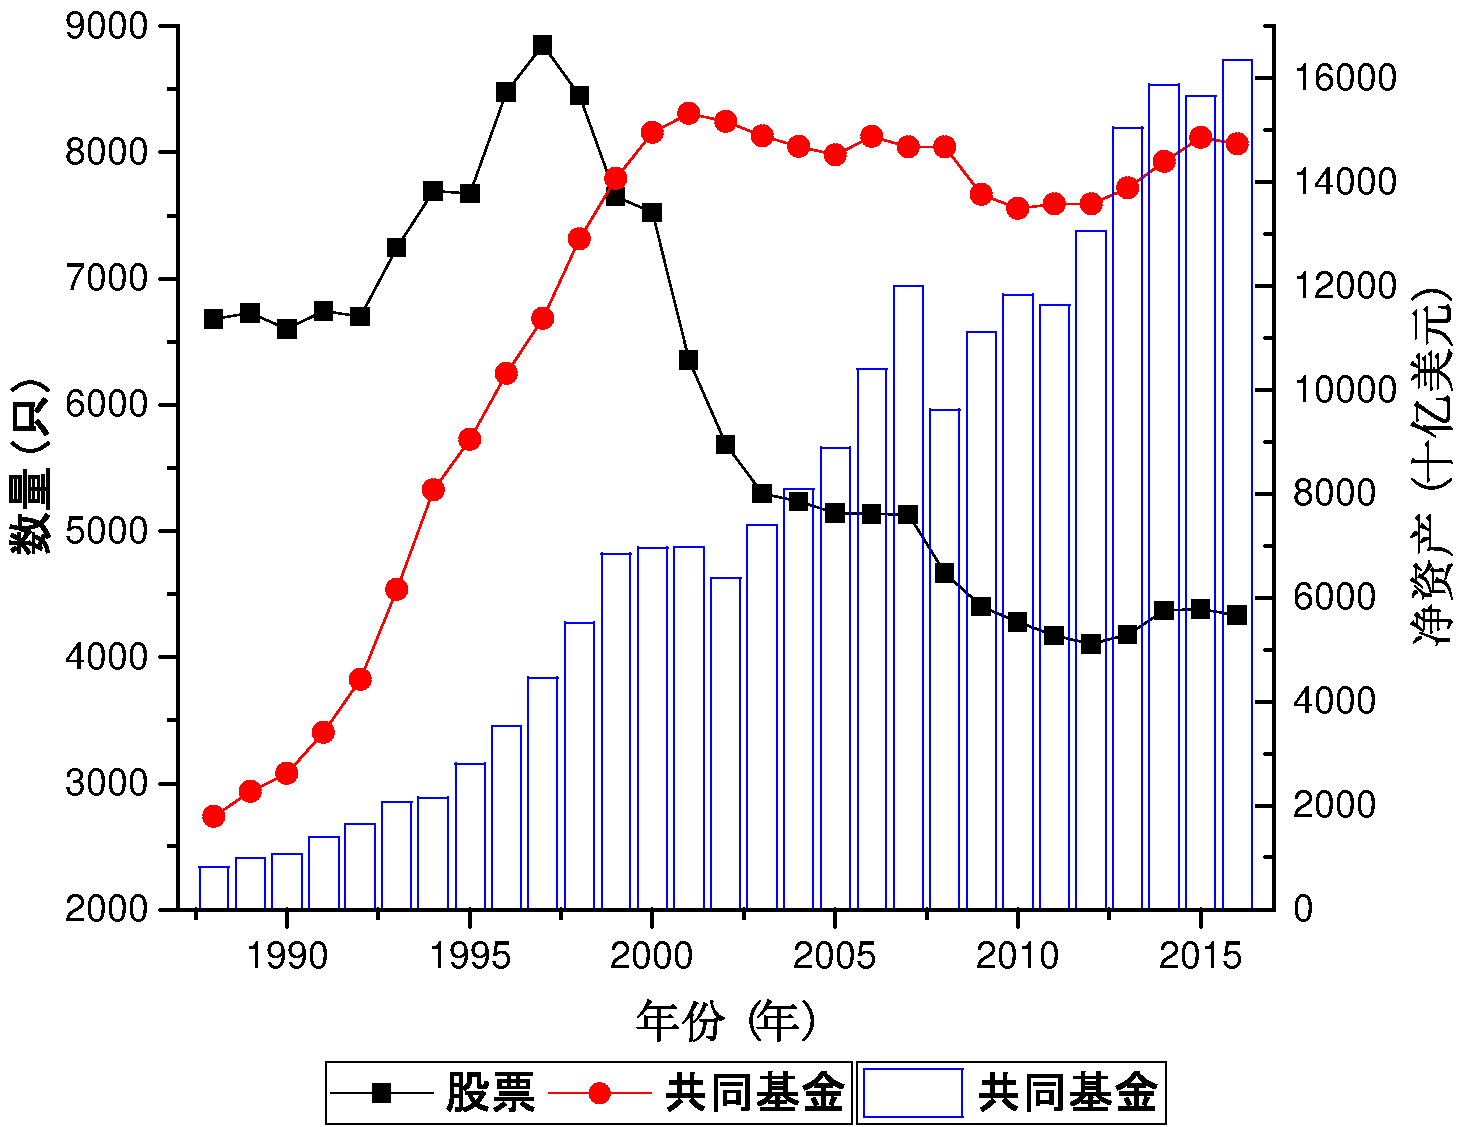
\includegraphics[width=\textwidth]{pic/mutual.pdf}
\subcaption{}\label{fg:mutual}
\end{minipage}%
\hspace{0.06\textwidth}
\begin{minipage}[ht]{0.47\textwidth}
\centering
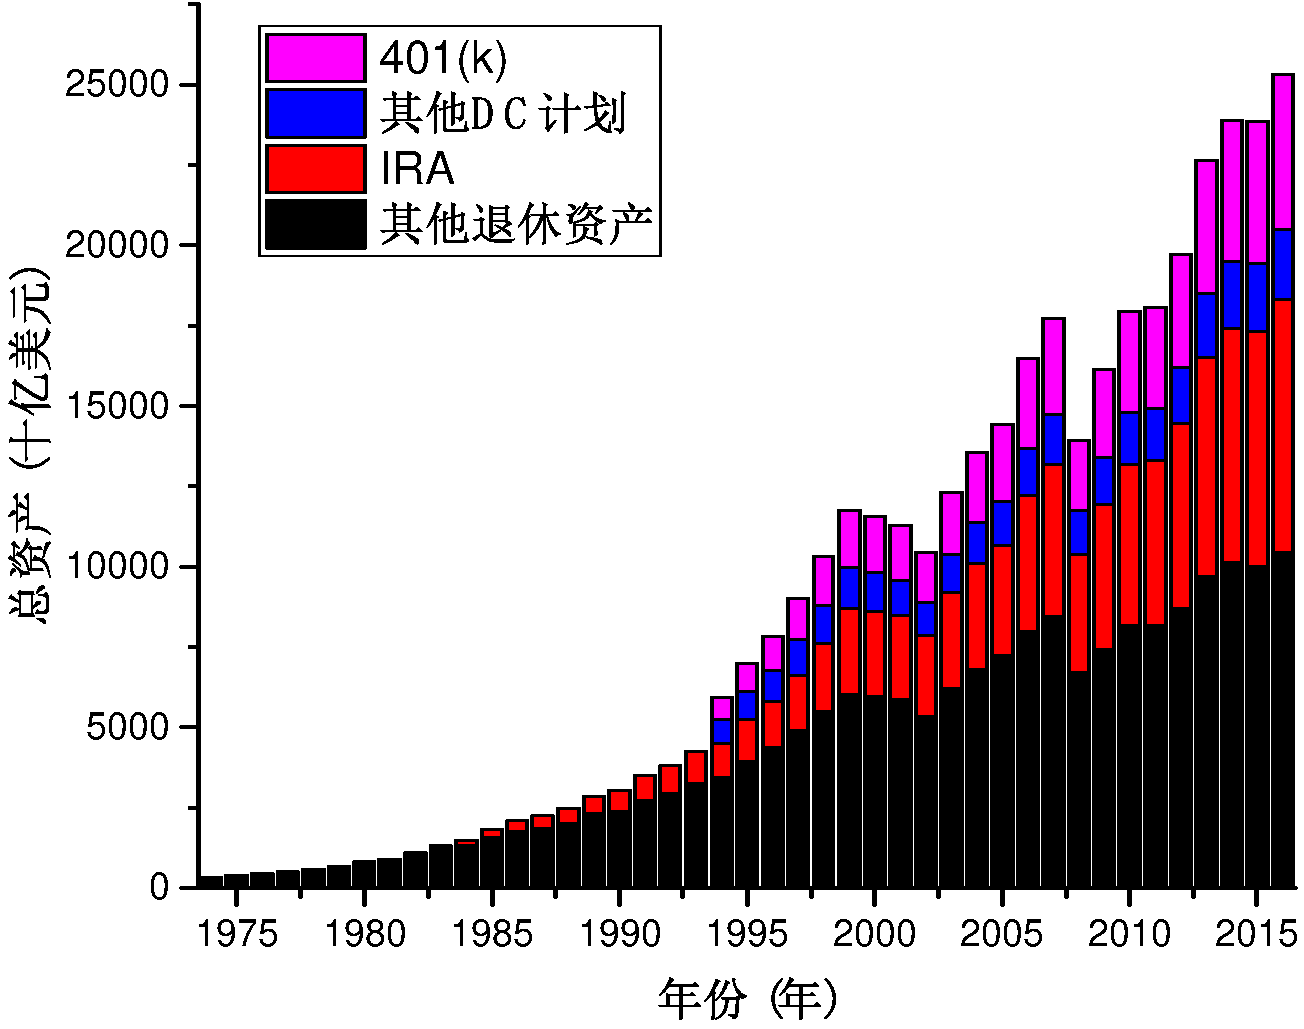
\includegraphics[width=\textwidth]{pic/retirement.pdf}
\subcaption{}\label{fg:retirement}
\end{minipage}
\caption{美国FOF基金相关市场发展:(a)1988--2016年美国股票、共同基金市场发展状况;(b)1974--2016年美国退休养老资产发展状况}
\end{figure}

共同基金在这次惨重的股灾过后,也不断开发出新的产品,基金的类型迅速增多,整个基金市场呈现爆发式增长,如图~\ref{fg:mutual}~所示,基金数量甚至远超股票数量.市场的复杂性、基金的多样性使得投资者对基金筛选及风险分散有了极大的需求,从此, FOF市场规模的扩大有了客观上的推动因素.

在同一时期,美国也大规模推广401(k)计划,这个计划的主要内容是创建了一个税收优惠账户,对雇员和雇主共同缴纳的养老金进行投资过程中收取的股息税和资本利得税进行减免.这为随后养老金进入资本市场打开了通道.

\subsection{基金中基金与养老金的关系\label{sec:retire}}

如上文所述,退休养老资产的扩大成为了美国基金中基金市场规模扩大的重要因素.为了能够吸引养老金投资者,基金公司推出了大量的针对养老金需求的基金中基金产品. 尽管FOF具有双重收费的劣势, 但它双重风险分散、多样化投资的优势吸引了大量养老金投资者的青睐.

退休养老基金主要投资于基金中基金产品,而基金中基金市场的主要资金来源也是退休养老基金,二者相互依存.基金中基金解决了养老金投资的难点,将两者紧密联系在一起.

\subsection{美国FOF市场的总资产序列}
根据彭博资讯提供的数据可以获取美国市场上所有FOF基金的规模及成立时间,以此统计出全市场的数量和规模,如图~\ref{fg:fof}~所示,时间区间为1995年1月至2017年5月,具体数据如表~\ref{tab:fof}~所示.
\begin{figure}[ht]
  \centering
  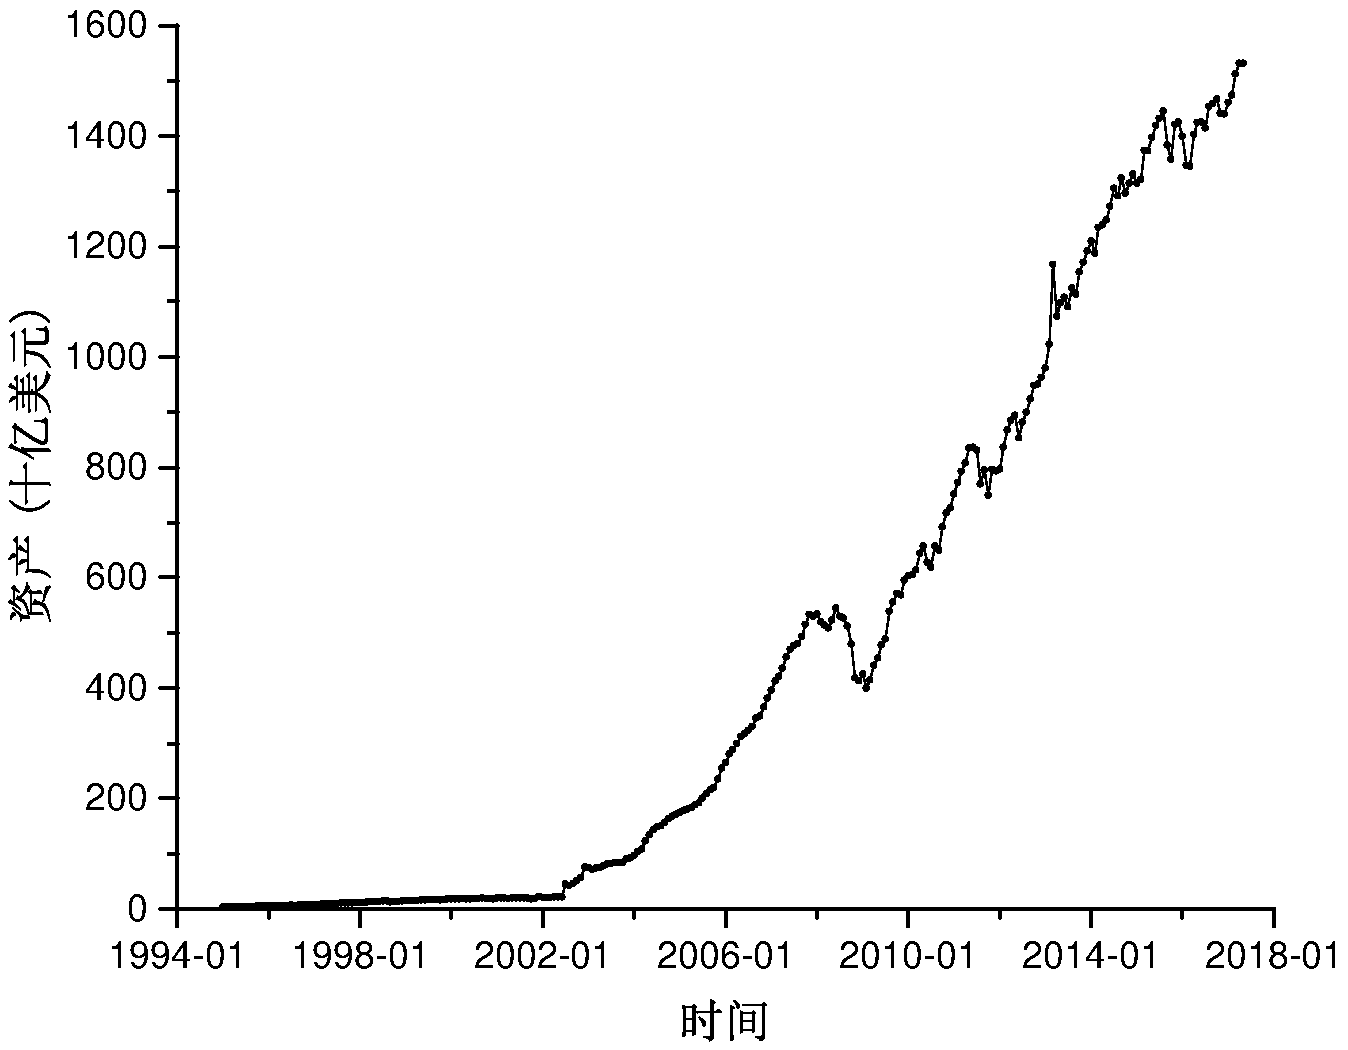
\includegraphics[width=0.6\textwidth]{pic/fof.pdf}
  \caption{1995年以来美国基金中基金市场的数量及规模}\label{fg:fof}
\end{figure}

如图~\ref{fg:fof}~所示,美国基金中基金市场的资产规模呈上升趋势,显示出明显的时间趋势.

\textcolor{red}{补充:把之前proposal中的数据描述,翻译成汉语,稍作修改,补充在这个地方,by王喆}

\textcolor{red}{修改:这部分引言是我自己写的,请二位提一提意见,然后我来修改,修改意见请二位单独写一个文件,或者像我一样加入红色的说明,否则的话容易被覆盖掉,by王喆\& RQJ}